%!TEX root = nextndnvideo-tr.tex
\section{prior work} % (fold)
\label{sec:comparison}
\begin{figure}%[htbp]
  \centering
  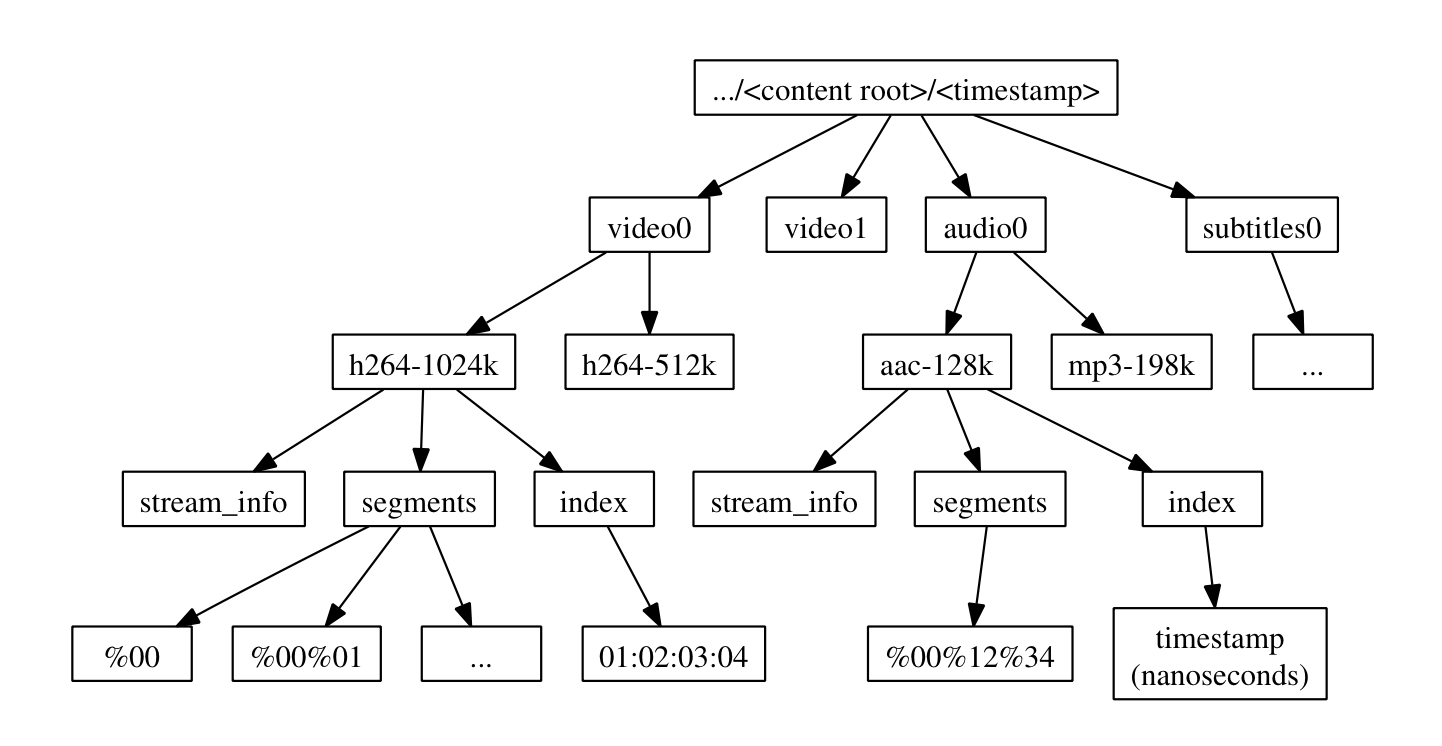
\includegraphics[scale=0.3]{ndnvideo_naming}
  % \vspace{-0.3cm}
  \caption{Prior NDNVideo Naming Space}
  \label{fig:ndnvideo_naming}
  %\vspace{-0.2cm}
\end{figure}
An similar work called NDNVideo was described in this technical report~\cite{ndnvideo}. Their aims are also to provide live and pre-recorded video streaming over NDN. They use Gstreamer to process media and Repo as the permanent storage. Producer and consumer concept are also the same, too. 

But the way how we handle framing are quite different. In the prior NDNVideo project, the video or audio stream is chopped into fixed size (segmentation) . A mapping between time and segment number is introduced to keep the video and audio synced (Figure~\ref{fig:ndnvideo_naming}). The seeking is also supported by the time-segment mapping mechanism. 

In our project, the video and audio is chopped into frames. One frame may contain several segments. The segmentation process is handled by Consumer / Producer API. The application only focuses on the frame level and leave other task to Consumer / Producer API. We think this application level framing is more like the true NDN way, which we mentioned in Section~\ref{sec:background}. Every frame has a unique name and is produced and consumed in one time. Only one frame missing won't affect other frames, thus leverage the whole impact to the playing back. 

On the contrary, the fixed size segmentation breaks the integrity of frames (ADU boundary). Only when all the packages are received correctly, the playing back progress can be guaranteed. So we think the prior NDNVideo is more like a TCP way. The application level framing also provides the flexibility to the video consumer. For example, in NDNLive, if the previous frame can't be retrieved on time or not integrated, the consumer can just skip this bad frame to keep the video streaming. We can see from the evaluation that it won't influence the video fluency. Table~\ref{table:comparison} shows other differences such as dependencies, Gstreamer version and coding language.

\begin{table}[ht]	
	\begin{tabular}{|c|c|c|}
	\hline
	             & NDNLive \& NDNTube                                                              & NDNVideo                                                     \\ \hline 
	Dependencies & \begin{tabular}[c]{@{}c@{}}ndn-cxx / NFD\\ Consumer / Producer API\end{tabular} & \begin{tabular}[c]{@{}c@{}}CCNx / CCNR \\ pyccn\end{tabular} \\ \hline
	Gstreamer    & 1.x                                                                             & 0.1                                                          \\ \hline
	Framing      & video \& audio frames                                                           & fixed segments                                               \\ \hline
	Language     & c++                                                                             & python                                                       \\ \hline
	\end{tabular}
	\caption{Comparison with NDNVideo}
	\label{table:comparison}
\end{table}
% section comparison (end)